\subsection{BLAS-like implementation}
Since the attempts to drive the compiler toward the best possible optimization failed, the last chance we have is to explicilty use \texttt{\textbf{AVX intrinsics}} to leverage the CPU's extended registers.

While the low-level implementation motivation are extensively explained in Appendix~\ref{subsec:openblas}, some tinkering with the code was needed to make it work with our use case. 

\subsubsection{Kernel $4\times8$}
In particular, the heart of the  algorithm is the \emph{kernel}, capable to work on multiple cells at the same time; we had to explicitly define it\footnote{In high-end libraries is directly written in Assembly or is written in a source code already "expanded" (i.e. with explicit unrolling, jamming, ...) by scripts that manages all edge-cases and hardware-dependent implementations.}.

\begin{lstlisting}[style=CStyle, caption={Kernel $4\times8$ doubles implementation},label={blas_like_code}]
static inline void kernel_4x8(int n, double (*C)[n], 
                              const double packedA_panel[KC][4], 
                              const double packedB_panel[KC][8], 
                              int kc, int i0, int j0) {
    __m256d c[4][2]; 
    #pragma unroll(4)
    for (int i = 0; i < 4; i++) { // Initialize accumulators
        c[i][0] = _mm256_setzero_pd();
        c[i][1] = _mm256_setzero_pd();
    }
    for (int p = 0; p < kc; p++) { //iterate over kc
        __m256d b0 = _mm256_load_pd(&packedB_panel[p][0]);
        __m256d b1 = _mm256_load_pd(&packedB_panel[p][4]);

        #pragma unroll(4)
        for (int i = 0; i < 4; i++) {
            __m256d a = _mm256_broadcast_sd(&packedA_panel[p][i]);
            c[i][0] = _mm256_fmadd_pd(a, b0, c[i][0]);
            c[i][1] = _mm256_fmadd_pd(a, b1, c[i][1]);
        }
    }
    #pragma unroll(4)
    for (int i = 0; i < 4; i++) {  // Update result matrix C
        __m256d orig0 = _mm256_load_pd(&C[i0 + i][j0 + 0]);
        __m256d orig1 = _mm256_load_pd(&C[i0 + i][j0 + 4]);
        _mm256_store_pd(&C[i0 + i][j0 + 0], _mm256_add_pd(orig0, c[i][0]));
        _mm256_store_pd(&C[i0 + i][j0 + 4], _mm256_add_pd(orig1, c[i][1]));
    }
}
\end{lstlisting}

 It calculates a $4 \times 8$ block of the destination matrix $C$ by multiplying a packed $4 \times kc$ panel of $A$ with a packed $kc \times 8$ panel of $B$. 

\paragraph{Optimization details}
This kernel is designed to fully utilize the capabilities of the AVX2 instruction set, which guarantees \texttt{\textbf{$16 \times$ 256-bit YMM}} registers. 

The kernel at any time keep a $4 \times 2$ array of \texttt{\_\_m256d} vectors. Since each vector holds four double-precision floating-point numbers, the 8 registers stores the 32 elements of the $4 \times 8$ target block of $C$.

By keeping the 8 accumulator registers, 2 registers for $B$, and 1 register for $A$ strictly in the CPU hardware, this kernel uses exactly 11 out of the 16 available \texttt{YMM} registers. This deliberate $4 \times 8$ sizing guarantees that all intermediate calculations occur without any costly "register spilling" to the L1 cache. 

After the iteration along the hidden dimension kc, the accumulated results are loaded, added to the original unaligned $C$ memory locations, and written back.

\paragraph{AVX Intrinsics Reference}
To achieve this low-level control, the kernel relies on Intel Intrinsic functions, which map directly to specific assembly instructions.

\begin{table}[H]
\centering
\caption{AVX2 Intrinsics used in the $4 \times 8$ kernel.}
\label{tab:avx_intrinsics}
\begin{tabular}{lp{10cm}}
\toprule
\textbf{Intrinsic Function} & \textbf{Hardware Operation} \\
\midrule
\texttt{\_\_m256d} & The underlying data type representing a 256-bit \texttt{YMM} register, that can holds 4 double-precision numbers. \\
\midrule
\texttt{\_mm256\_setzero\_pd()} & Returns a 256-bit vector with all bits set to zero.\\
\midrule
\texttt{\_mm256\_load\_pd(ptr)} & Loads 4 packed double-precision values from memory into a vector.\\
\midrule
\texttt{\_mm256\_broadcast\_sd(ptr)} & Loads a single double-precision value from memory and duplicates (broadcasts) it across all 4 elements of the destination vector. \\
\midrule
\texttt{\_mm256\_fmadd\_pd(a, b, c)} & Performs a Fused Multiply-Add operation. It computes $(a \times b) + c$ for all 4 packed elements simultaneously, maintaining infinite intermediate precision before rounding. \\
\midrule
\texttt{\_mm256\_add\_pd(a, b)} & Performs a standard element-wise addition of two 256-bit vectors containing double-precision values. \\
\midrule
\texttt{\_mm256\_storeu\_pd(ptr, a)} & Stores 4 double-precision values from a vector into a  memory location.\\
\bottomrule
\end{tabular}
\end{table}

\paragraph{Hyperparameter tuning}
The algorithm requires tuning the tiling dimensions \texttt{\textbf{MC, NC}}, and \texttt{\textbf{KC}}. The static kernel size ($N_R = 8$, $M_R = 4$), along with the simplification implemented imposes strict alignment constraints: $K_C$ and $N_C$ must be multiples of 8, and $M_C$ must be a multiple of 4.

While theoretical upper bounds can be calculated based on the hardware cache limits in Table~\ref{tab:cache_partitioning}, dictates that the dimensions must be carefully balanced to prevent L2 cache eviction\footnote{The constraints are that: (1) $K_C \times N_R$ elements must fit within the L1 cache; (2) $M_C \times K_C$ elements must fit within the L2 cache, and (3) $N_C \times K_C$ elements must fit within the L3 cache.}.

In the end, rather than relying solely on theoretical maximums, we conducted an empirical search over various block-sized configurations, finding the best-performing tuple defined by $$\texttt{\(\textbf{MC=256, NC=512, KC=256}\)}$$

\paragraph{What is missing from the original}

Compared to the official \texttt{OpenBLAS} library, our custom implementation performs a little worse (ee Figure~\ref{fig:openblas_vs_blas_roofline}). This is mainly caused by the fact that the highly optimized \texttt{OpenBLAS} architecture utilizes a $6 \times 8$ kernel (that obviously performs better, since it uses more registers). 

However, as detailed in Appendix~\ref{subsec:openblas}, by using a $6 \times 8$ kernel significant implementation hazards arises, since the kernel must also work on the  edge of the matrices.

By opting for a $4 \times 8$ kernel and by constraining the use of our \texttt{-DALIGN} padding strategy, we avoid altogether these complications. Because our matrices are explicitly padded to ensure their dimension $n'$ is always a multiple of 8, the $4 \times 8$ kernel inherently divides the iteration space evenly.

\subsubsection{Performances evaluation}
To verify the effectiveness of our implementation we directly compare it with the original one from \texttt{openBLAS}, using once again Intel Advisor.

\begin{figure}[H]
\centering
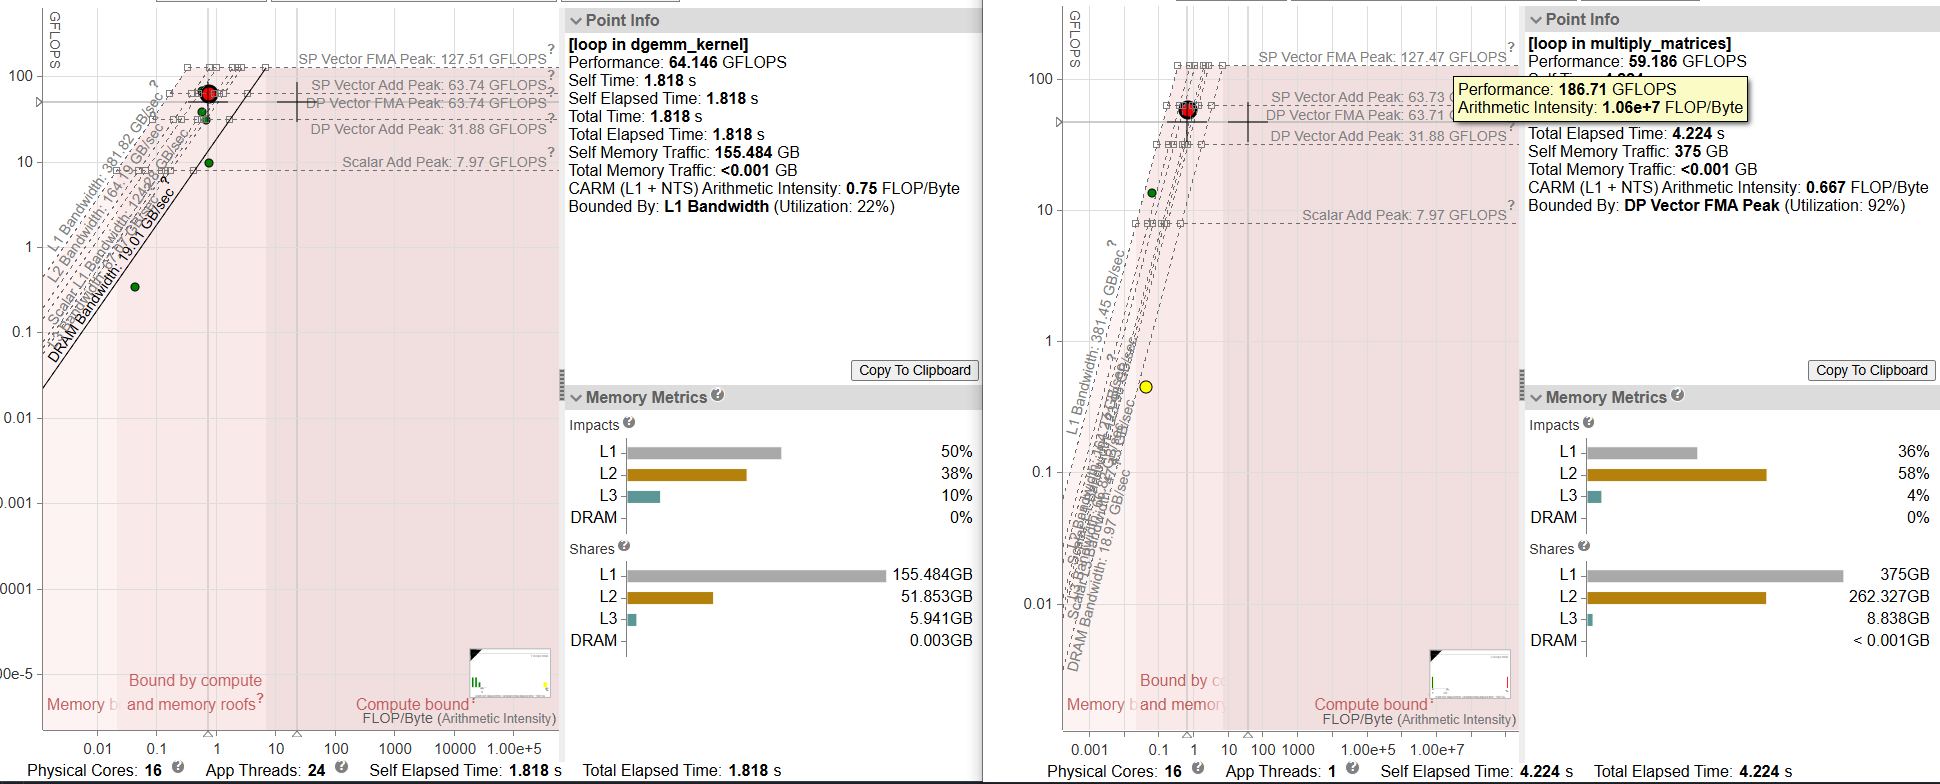
\includegraphics[width=1\textwidth]{Images/openblas_vs_blas_roofline.png}
\caption{Roofline comparison between the original \texttt{OpenBLAS} (left) and our custom implementation (right).}
\label{fig:openblas_vs_blas_roofline}
\end{figure}

As expected, the original \texttt{OpenBLAS} implementation achieves a slightly higher throughput of \textbf{64.146 GFLOPS}. It is classified as bounded by \textbf{L1 Bandwidth}, saturating it with a higher Arithmetic Intensity of $0.75$ FLOP/Byte; there is very little room left for optimization on the machine.

On the other hand, our custom $4 \times 8$ implementation is bounded by the \textbf{DP Vector FMA Peak}, reaching \textbf{59.186 GFLOPS}.As highlighted before, since we use a $4 \times 8$ micro-kernel instead of the $6 \times 8$ one used by OpenBLAS, we do not fully fill all available SIMD registers, hence shifting the primary bottleneck from the memory subsystem (L1 bandwidth) directly to the execution units.

\paragraph{Broader comparison}
The final results are shown in Figure~\ref{fig:blas_vs_openblas}.

\begin{figure}[H]
\centering
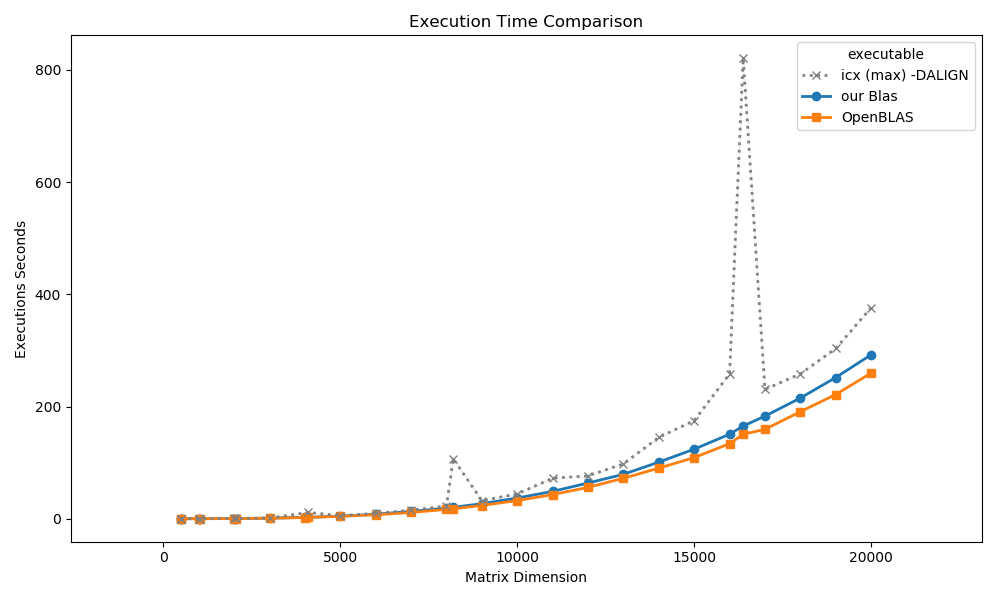
\includegraphics[width=0.8\textwidth]{Images/blas_vs_openblas.png}
\caption{Performance comparison of the original \texttt{OpenBLAS} and our custom implementation 
}
\label{fig:blas_vs_openblas}
\end{figure}

The plot clearly shows a smooth, cubic trends that \emph{finally} matches the suggested complexity of $O(n^3)$, and the already discussed  supremacy of the original version. 

We can now consider completed the quest of the search for the best possible sequential implementation.
